\section{The URDAD metamodel \label{sec:metamodel}}

In an effort to formalize URDAD, there exists a need for the formal specification of URDAD's concepts and the rules associated with the use of the URDAD methodology. To this end we define a metamodel. A metamodel is the ``logical information model that specifies the modeling elements used within another (or the same) modeling notation'' \cite{_ieee_2003}. The URDAD metamodel formalizes the modeling constructs required by the URDAD methodology to store the requirements for a service and the technology neutral design of a business process realizing these requirements\footnote{In adition metamodel, the URDAD-DSL comes with standard library specififying primitive data types, entities and core persistence services.}. 

Metamodels are closely related to ontologies. Both provide a way to define concepts and relationships between concepts. For practicality reasons, the semantics has been encoded in EMOF/Ecore instead of {\em Web Ontology Language}, OWL\cite{zuo_zhihong_web_2003}. It is motivated by the technology support for developing a concrete textual and graphical syntax for the DSL \cite{heidenreich_derivation_2009}, the support for model-to-model \cite{_meta_2011} and model-to-text transformations \cite{model2text} and the availability of OCL as a constraint language \cite{OCL} for querying model instances and for specifying constraints at both, the metamodel and model levels. Mappings between these two technologies can be readily performed \cite{staab_model_2010}. A transformation to OWL facilitates reasoning services like consistency and completeness assessment.

The URDAD metamodel provides a minimalistic set of modeling constructs for services oriented analysis and design. It facilitates the recursive decomposition of service requirements into lower level services requirements with pre- and post-conditions as well as quality requirements for each service and the data structure specifications for the inputs and outputs and the process specification on how a service is orchestrated across lower level services. 


The URDAD metamodel has been strongly influenced by the Unified Modeling Language, UML, in the areas of data structure specification and by service-oriented process specification languages like the Business Process Execution Language, BPEL, in the areas of process specification. 
It enforces assembly of higher level stateless services from lower level stateless services with the leaf services sourced from the environment (e.g.\ from the programming language, libraries, frameworks and automated and non-automated external service providers). 

The URDAD DSL is, however, a fraction of the size of the UML, yet adds some core concepts required by the URDAD methodology including (1) a higher-level constraint infrastructure supporting parametrized, reusable constraints which are assessed through processes extracting information from the environment, (2) explicit modelling constructs for specifying a services contract (3) relationships facilitating improved traceability, (3) the concept of a responsibility domain, (4) association of exceptions to pre-conditions, (4)
the separation of the identification of a resource (object or service) from a path to it, (5) enforcing service-specific request and result classes and (6) enforcing that a service either yields the result or notifies the user that the service is not provided due to a pre-condition not having been met.

%--------------------------

\subsection{URDAD-DSL core}

The core modules introduces the concept of the model, model elements and stakeholders, responsibility domains, expressions and annotations. Most of these are self-explanatory. The URDAD-DSL does not lock into any particular expression language (e.g.\ the language to specify constraint expressions). 

\begin{figure}[Htb]
  \centering
  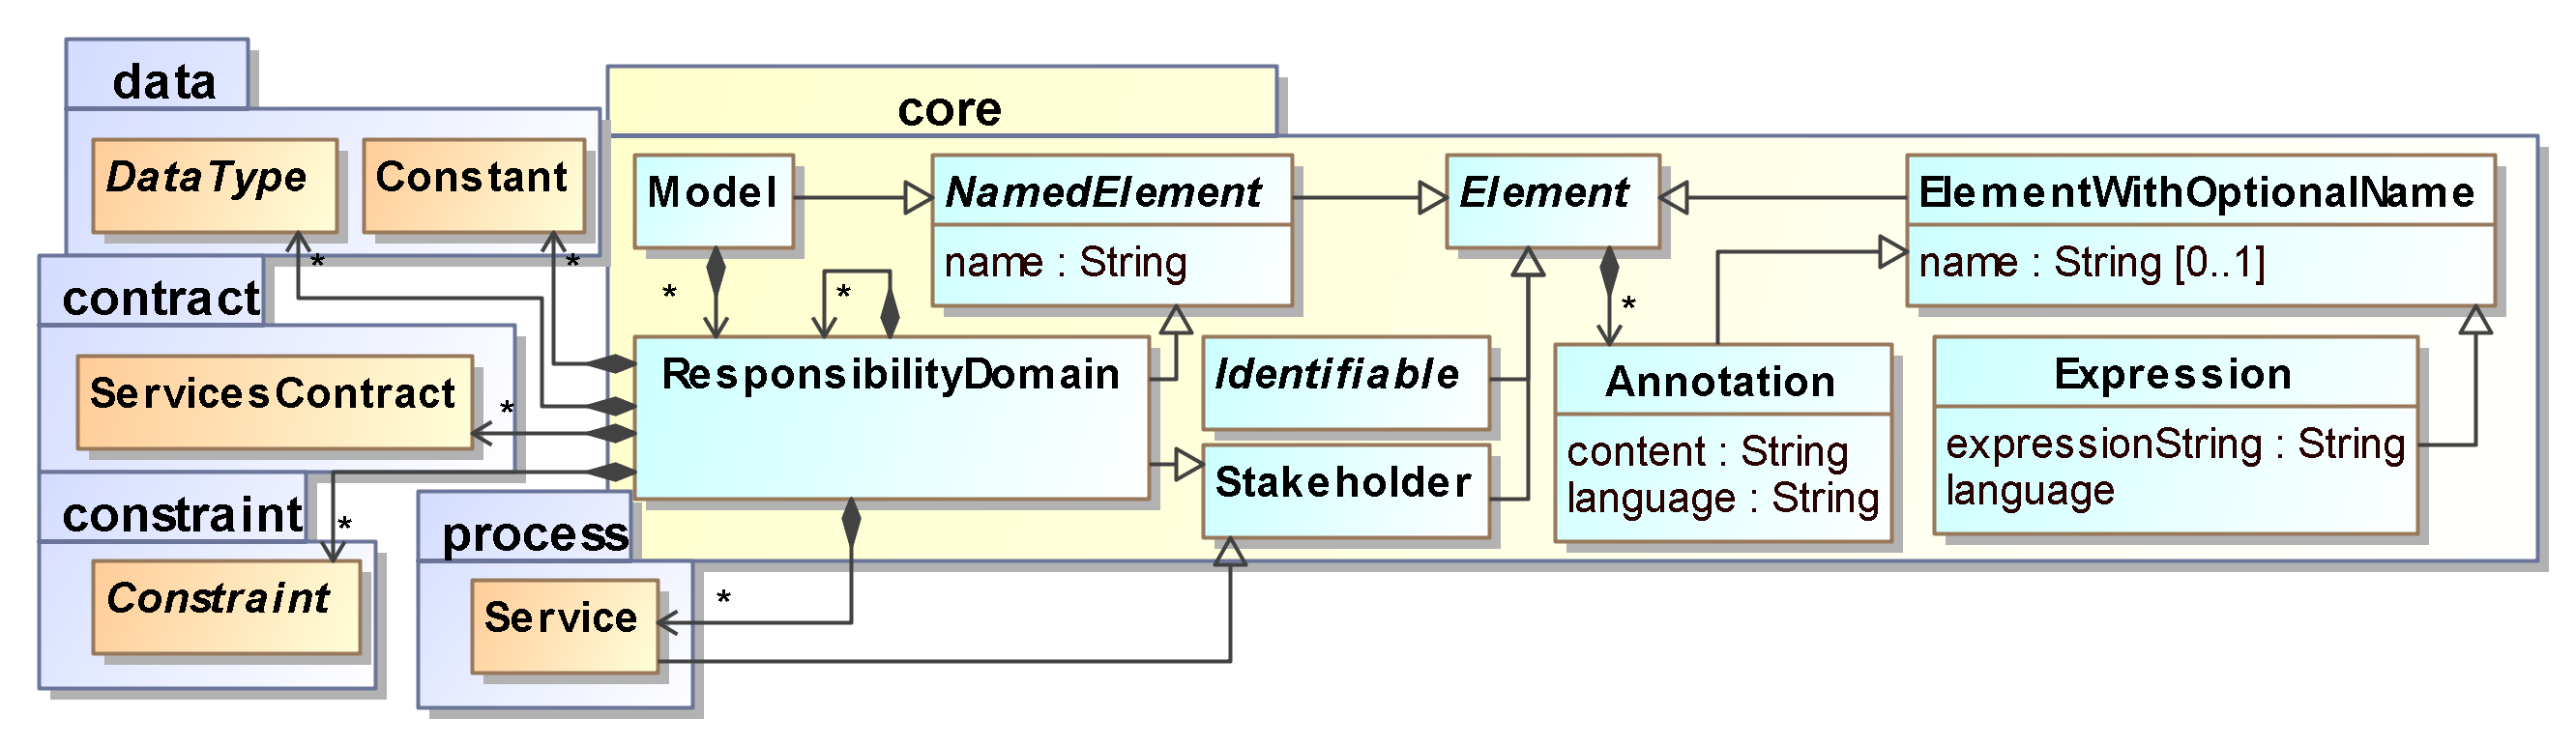
\includegraphics{core}
  \caption{The core elements of URDAD}
  \label{fig:metamodel}
\end{figure}

Responsibility domains represent the important concept of a role in URDAD. A physical resource (person, system, module, \dots) may be assigned one or more responsibility domains. A responsibility domain covers a cohesive unit of functionality at a particular level of granularity. For example, there may be a finance responsibility and within it there are lower level responsibility domains like creditors and debtors.  Responsibility domains are closely related to the concept of unity criteria \cite{gonzalez_unity_2009}. They represents groupings of cohesive services contracts and eliminate the need for the separate definition of a services provider contract which encapsulates the services contracts for different services of a particular responsibility domain. Note that a responsibility domain defines the boundaries between levels of granularity with lower level granularity services of a responsibility domain being contained in lower level responsibility domains. Technically a responsibility domain provides packaging construct associating model elements with a unique name space.

Every requirement needs to be required by at least one stakeholder which is either a responsibility domain (e.g.\ user, industry regulator, finance, \dots) or a particular service realization (if we realize the service in this way we require that a lower level service which realizes that services contract).


%--------------------------

\subsection{Constraints}

The Object-Constraint Language (OCL) has become the de-facto standard for specifying constraints across object graphs \cite{_object_2010}. However, in a services oriented approach and in the context of reusable, parametrized constraints, OCL alone is insufficient.
Reusable constraints require support for binding parameters. For example, one might have a constraint that a person is registered. This constraint can be used in the context of pre-conditions for certain services and is most likely a post-condition for the registration service itself. However, the person identifier would have to be passed as a parameter to the constraint if the constraint is to be widely reusable.

The second reason for having to add additional constraint infrastructure to the URDAD-DSL is that in a services oriented world the actual environmental state is not directly specified, but accessible only via services. In such a world it is not possible to specify testable constraints via a pure constraint language like OCL. The constraint specification needs to include the specification of services which are used to obtain the state information and the associated service request object. The construction of these request objects might itself even require a process where the information is obtained from the environment. The  URDAD-DSL constraint specification includes the specification a process to source information from the environment together with a set of constraints which apply to that information. Having sourced the information from the environment, OCL or another constraint specification language (the metamodel does not prescribe the constraint specification language) can be used to specify the constraints which apply to the obtained information.

\begin{figure}[Htbp]
  \centering
  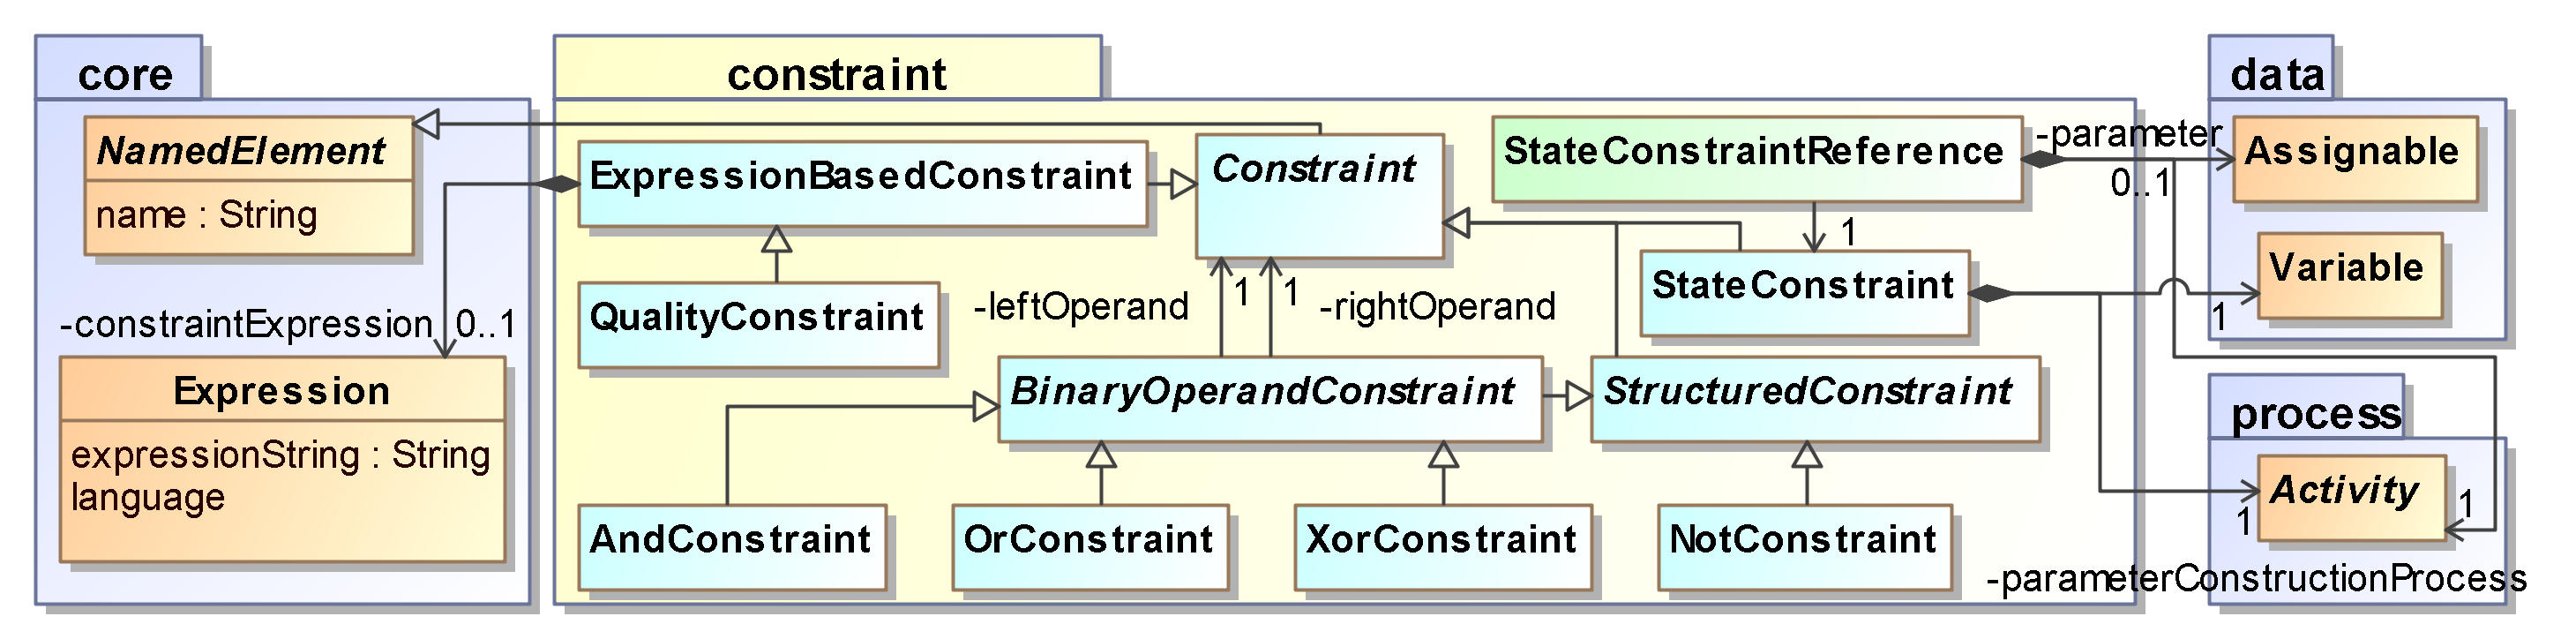
\includegraphics{constraint}
  \caption{The constraint specification elements of URDAD}
  \label{fig:metamodel}
\end{figure}

The constraints module provides the concept of re-usable constraints. Parametrized state constraints are assembled from a process querying the environment and a set of constraints on the information obtained from the environment. A state constraint reference has the option to include a constraint parameter as well as the specification of a process to construct that parameter. The module also contains a set of standard logical operators enabling one to assemble higher-level constraints from lower level constraints.

%--------------------------

\subsection{Services contracts}

The core of the contracts package is a services contract with both, functional requirements (pre- and post-conditions) and quality requirements. Each requirement is associated with a a stakeholder which is either a responsibility domain (role) or another service which introduces that requirement. 

A pre-condition is a condition under which the service provider may refuse the service without the refusal of service implying a breach of the services contract. The specification of a pre-condition includes the identification of the exception which is used to notify a service user that the requested service was not provided due to a particular pre-condition not having been met. A post-condition, on the other hand, is a condition which holds true after the service has been provided. It is either a condition on the result or on the change in the state of the environment of the service. Due to a service potentially resulting in a lasting change to its environment, the URDAD-DSL allows the designation of an inverse service through which that lasting effect can be reversed. This enables the automatic reversal of a partially completed process by calling the inverse services of those lower level services which have thus far been completed within the process.

Functional requirements may be conditional and are bound to reusable state constraints.  Quality requirements are bound to quality constraints.

\begin{figure}[Htbp]
  \centering
  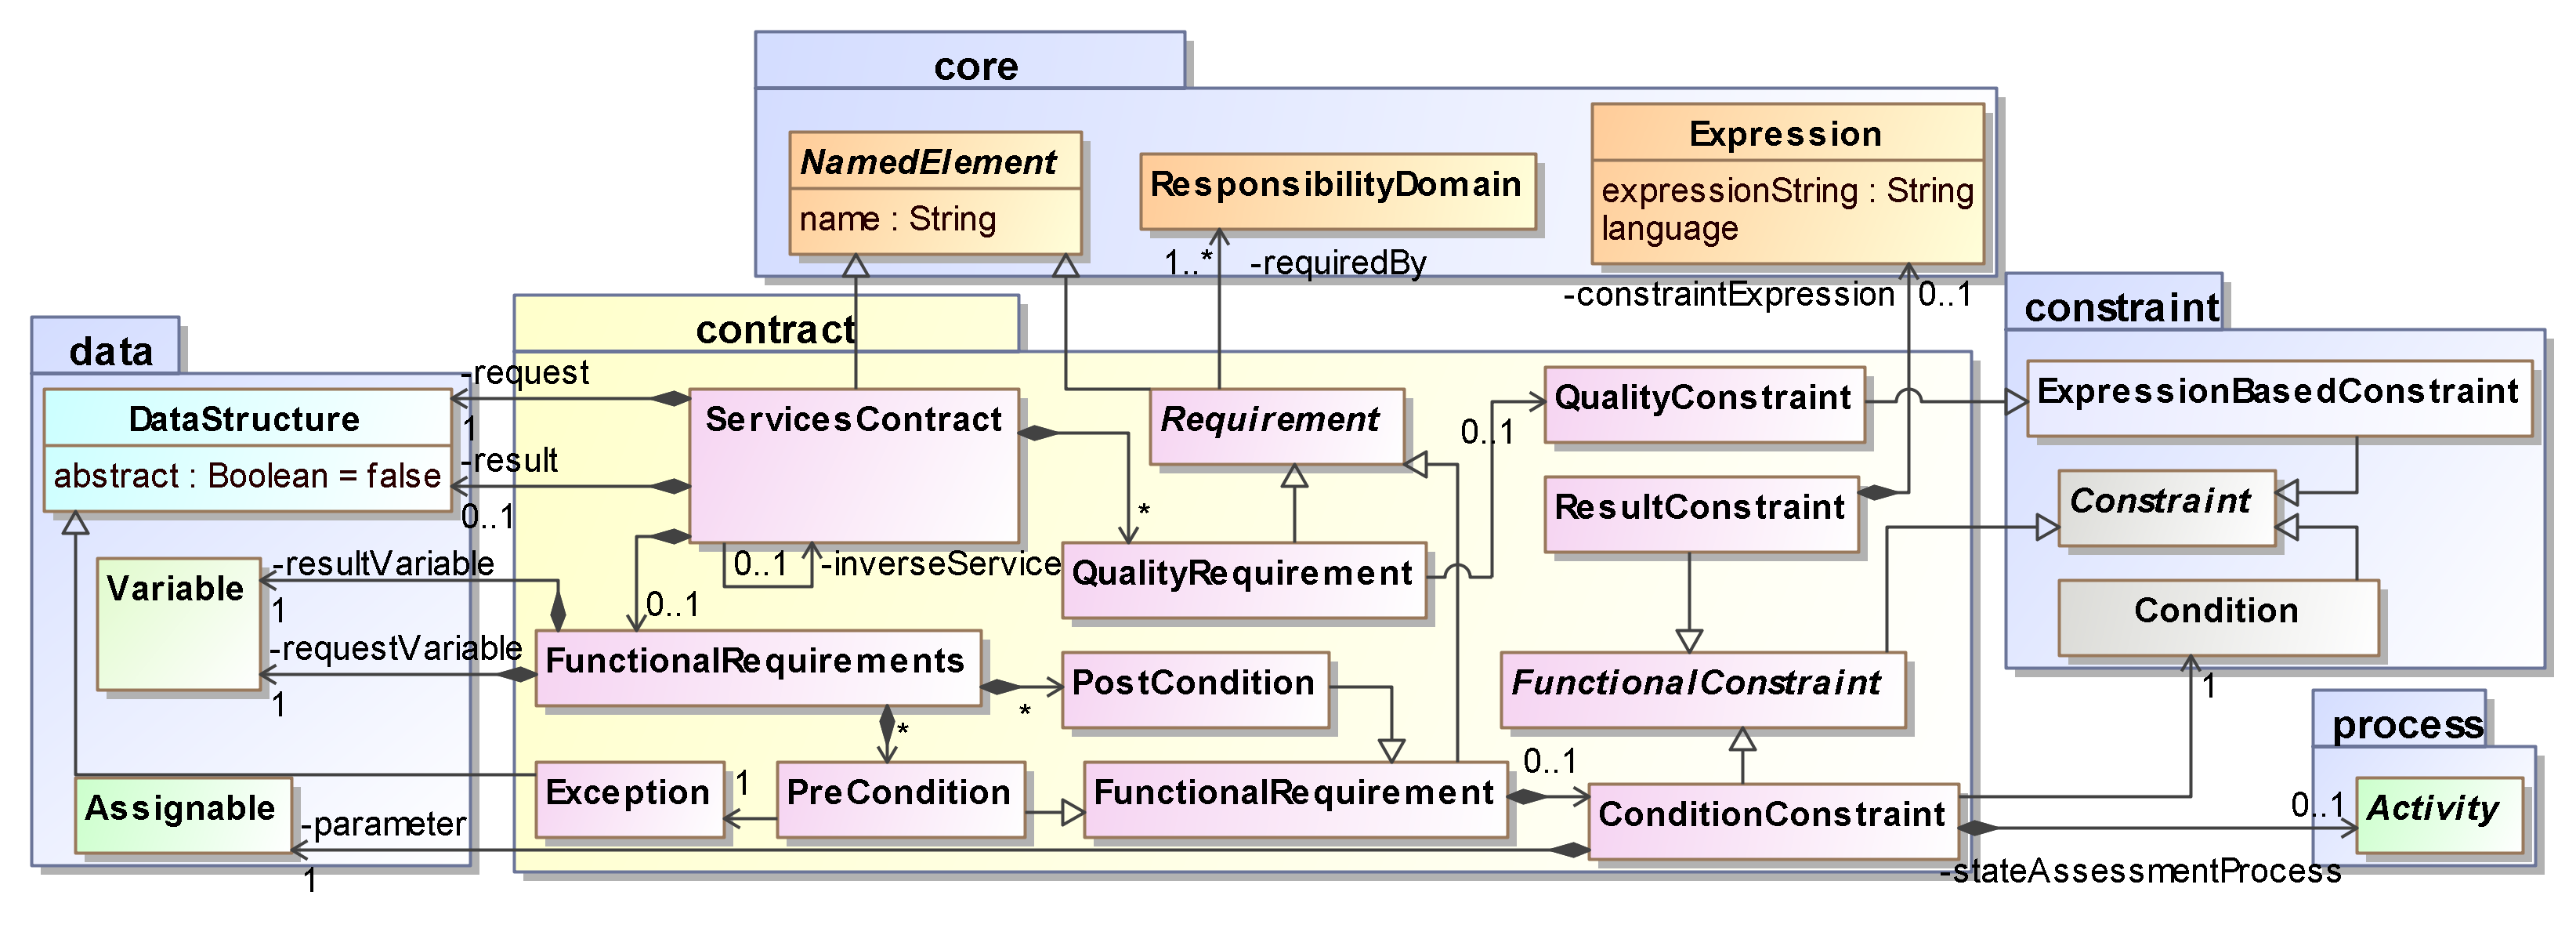
\includegraphics{contract}
  \caption{The contract specification elements of URDAD}
  \label{fig:metamodel}
\end{figure}

A services contract specifies a single service request object that contains detailed information pertaining to the request and a single result object, which is composed of the information associated with the result of the service execution. The data structures for these request and result objects are service specific and are not meant to be reused, even though their components are commonly domain objects which are widely reused. They are thus specified within the services contract and are named \verb+<ServiceName>Request+ and \verb+ServiceName+Result.


%--------------------------

\begin{figure}[Htbp]
  \centering
  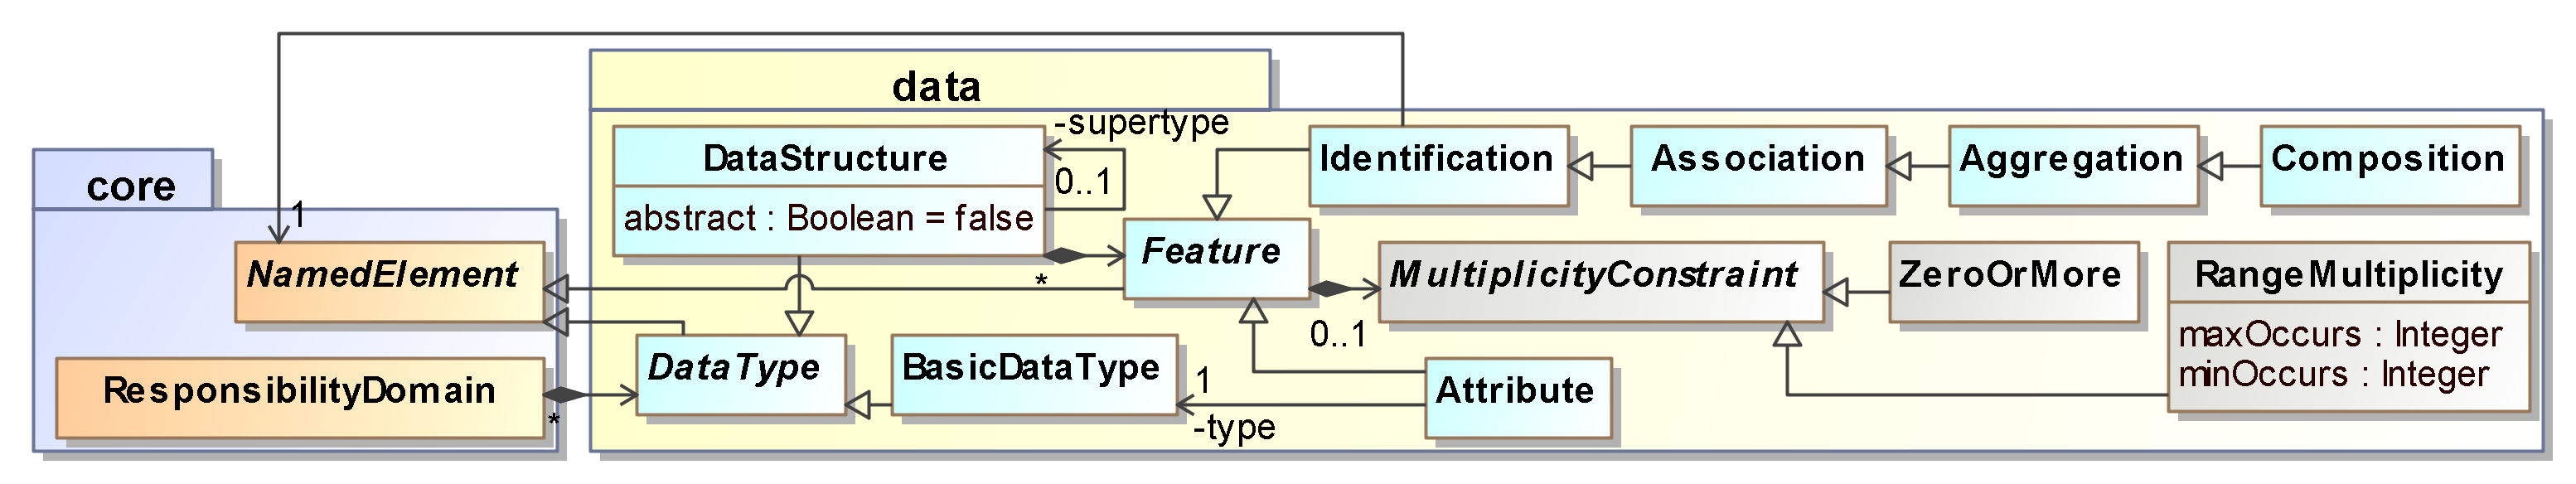
\includegraphics{data}
  \caption{The data definition elements of URDAD}
  \label{fig:metamodel}
\end{figure}

\subsection{Data structures}

The data module is a standard object-oriented approach to data structure specification similar to UML class models. The core additions are that of separating an identification from an association and the concept of an assignable which can be a variable (object), variable reference, query or constant. An identification purely identifies a resource (object or service), relying on the environment to be able to source the resource from the environment. It is an abstraction of the concept of a \emph{Uniform Resource Identifier} (URI). An association, on the hand, resembles a path to the resource.

%--------------------------
\begin{figure}[Htbp]
  \centering
  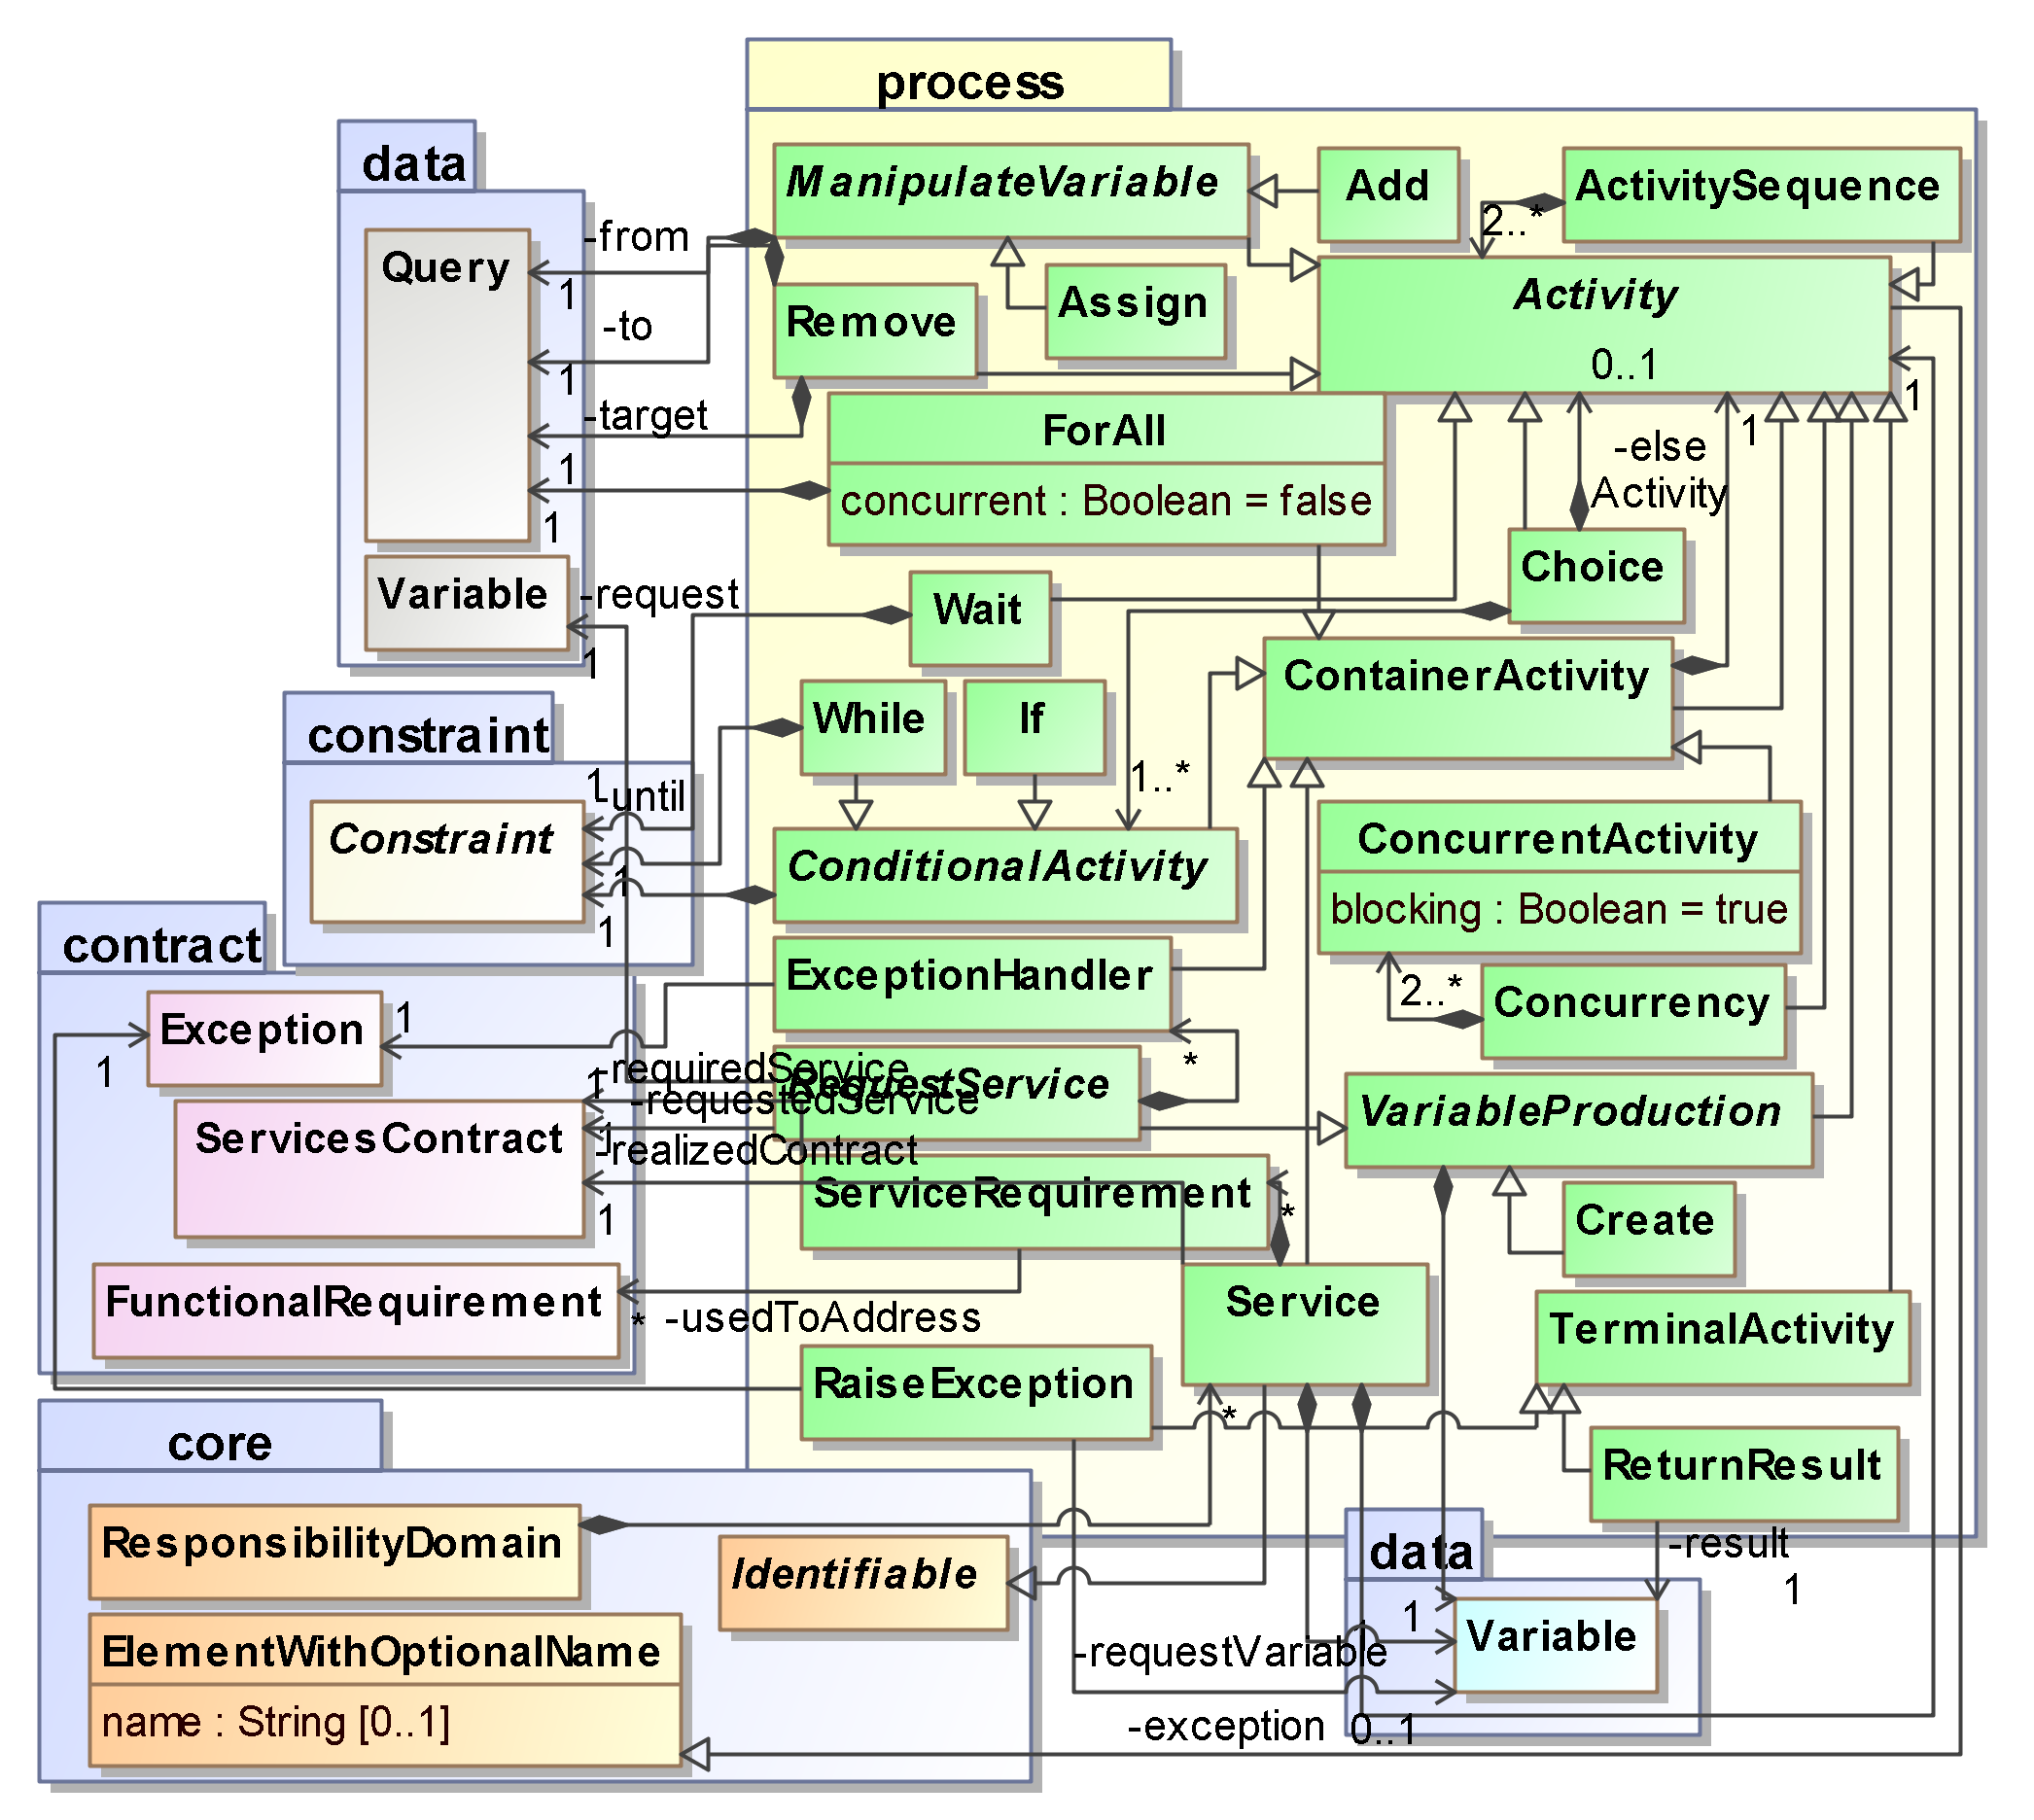
\includegraphics{process}
  \caption{The process definition elements of URDAD}
  \label{fig:metamodel}
\end{figure}

\subsection{Processes}

The process package introduces the concept of a service which is a concrete unit of functionality realizing a services contract. For a service one species the lower level services used to address the different pre- and post-conditions. This requirement of the URDAD methodology improves traceability providing satisfaction links discussed in \cite{ramesh_toward_2001}). Each activity within the service process is associated with either (1) the maintenance of local process variables, (2) the validation of a pre-condition and/or the fulfillment of a post-condition through the execution of a lower level service, (3) the handling of an exception received from a lower level service, (4) the raising of an exception or the return of the result.

The URDAD methodology enforces decoupling through services contracts. This is  enforced in the URDAD metamodel by linking both, satisfaction links and service requests to service contracts and not concrete services. Note also that URDAD assumes that the concrete services used to realize the services contracts are specified either during implementation mapping or by the run-time environment and not in the technology neutral model. They could, for example, be injected by the run-time environment like in Spring or Java-EE based dependency injection.

An important non-functional requirement of all activities that constitute a service's process, is that each activity must be traceable back to the fulfillment of one or more of the functional requirements. There should be no redundancy and only the functional requirements that are associated with the service should be addressed by the process.


